\section{Performance} % (fold)
A summary of all methods is plotted in \ref{fig:chargesummary} and \ref{fig:penumsummary}. Figure \label{fig:chargesummary} is reconstruction of charge. Figure \label{fig:penumsummary} is reconstruction of \#PE. The errorbar shows 10 to 90 percentile of Wasserstein distance. 

\begin{figure}[H]
\begin{minipage}{.5\textwidth}
\begin{figure}[H]
    \centering
    \caption{Distances of methods, error bar 10 - 90 percentile (Charge)}
    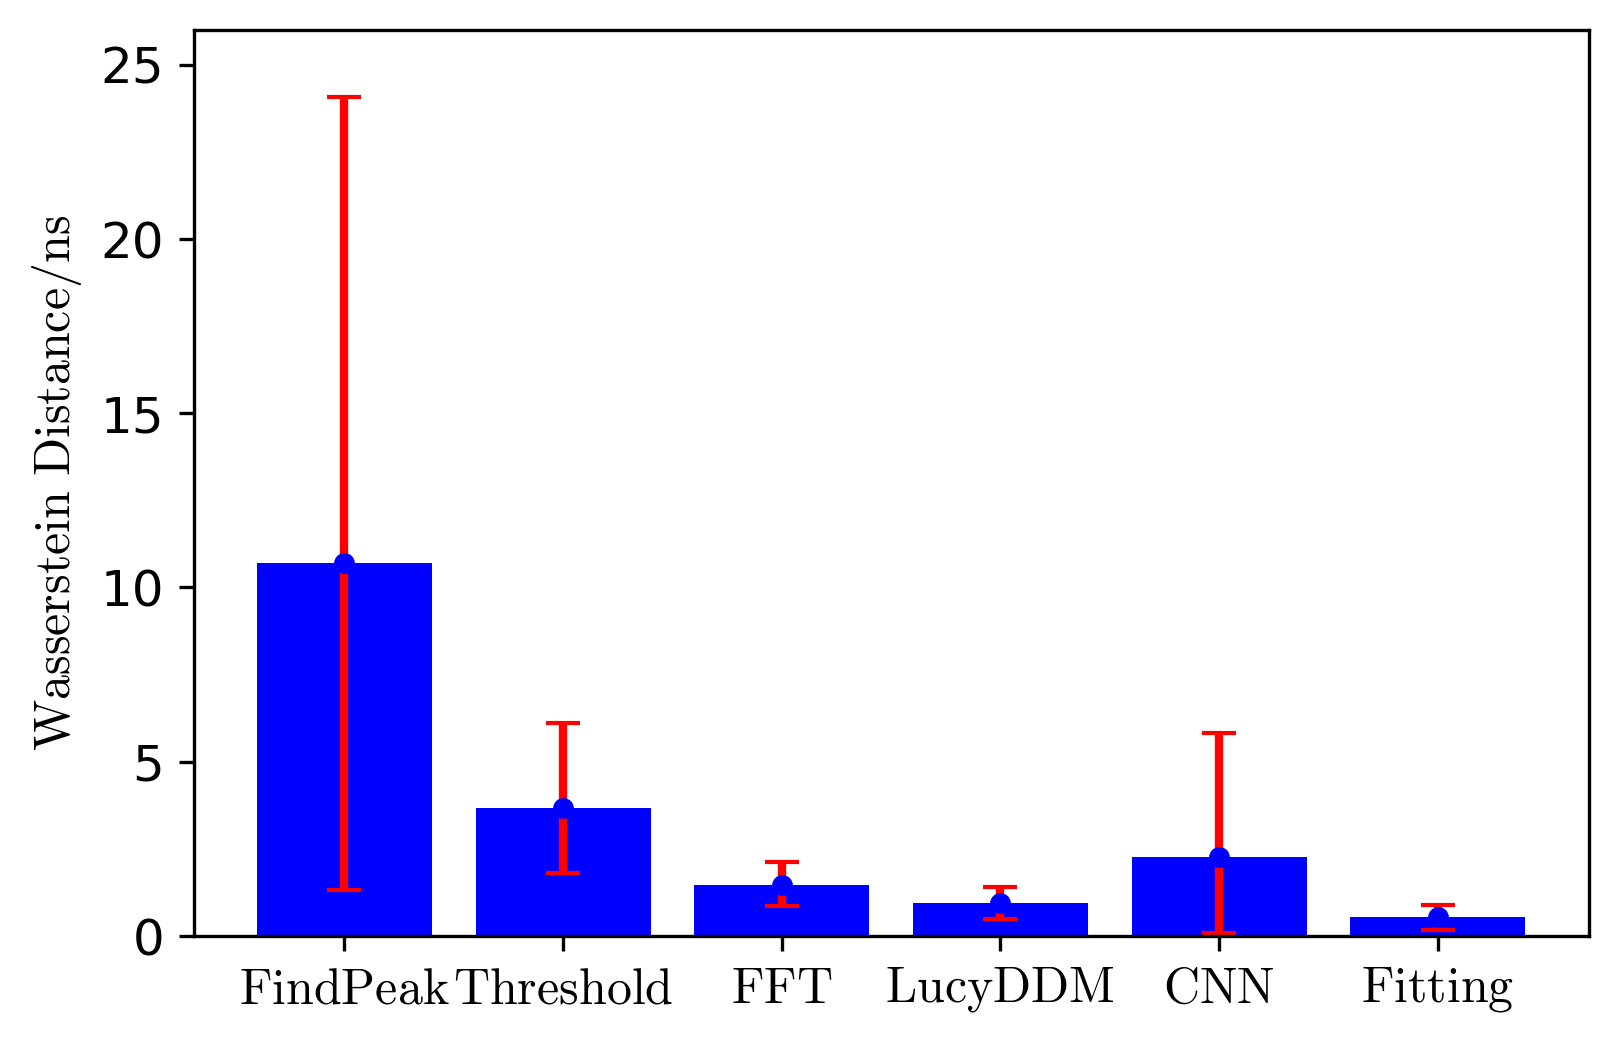
\includegraphics[width=1.0\linewidth]{figures/summarycharge.png}
    \label{fig:chargesummary}
\end{figure}
\end{minipage}
\begin{minipage}{.5\textwidth}
\begin{figure}[H]
    \centering
    \caption{Distances of methods, error bar 10 - 90 percentile (\#PE)}
    \includegraphics[width=1.0\linewidth]{figures/summarypenum.png}
    \label{fig:penumsummary}
\end{figure}
\end{minipage}
\end{figure}

The efficiency of CNN fitting and Lucy deconvolution method show in Table \ref{fig:efficiency}. The CNN is faster than Lucy deconvolution, and much faster than fitting.  

\begin{table}[H]
    \centering
    \caption{Reconstruction Efficiency}
    \begin{tabular}{c|c|c}
        \hline
        &  & Performance/$10^{5}$Waveform \\
        \hline
        CNN & Charge & 6.0s (GPU) \\
        \hline
        CNN & \#PE & 6.0s (GPU)\\
        \hline
        Fitting & Charge & 2000s (CPU) \\
        \hline
        Fitting & \#PE & 2000s (CPU) \\
        \hline
        LucyDDM & Charge & 24s (CPU) \\
        \hline
        LucyDDM & \#PE & 24s (CPU) \\
        \hline
    \end{tabular}
    \label{fig:efficiency}
\end{table}
\hspace{4mm}
\begin{center}
\begin{itemize}
    \item GPU: Using one graphic card of NVIDIA Tesla K80
    \item CPU: Using 50 CPU cores of AMD EYPC 7702
\end{itemize}
\end{center}

% section Performance (end)